\documentclass[a4paper,10pt]{article}
\usepackage[utf8]{inputenc}
\usepackage{graphicx}
\usepackage{framed} 
\usepackage{xcolor}
\usepackage{tcolorbox}
\usepackage{xcolor} 
\colorlet{shadecolor}{gray!25}
\definecolor{mshadecolor}{rgb}{0.7421875,0.7421875,0.7421875}

%opening
\title{Offensive Security\\
	Lab-report
}
\author{Moritz Rupp}
\begin{document}

\maketitle
\tableofcontents
\begin{abstract}
Lab3 documentation
\end{abstract}
\newpage
\section{Exercise 3}
\subsection{UART Communication Analysis}
Salea offers an extension 'Saleae-Hex-Ascii-Dec-to-Terminal` that is capable of converting low level analyser output to human readable data. This way we can write the bewished encoding like ascii to a file of choice.\\
With the help of a simple Python script, it's now possible to read out the flag.
\begin{center}
 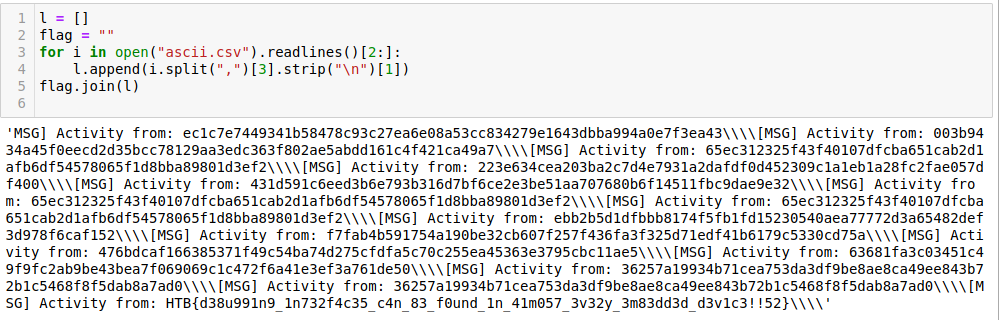
\includegraphics[scale=0.4]{3.1.png}
\end{center}
\subsection{Binary Data Analaysis}
Using the shell commands 'file' we discover that the provided image is an 'Linux kernel ARM boot executable zImage'. After some research we are able to extract all contents of the Image.
\begin{center}
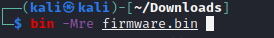
\includegraphics[scale=0.6]{binwalk.png}
\end{center}
This resulted in a folder '\_firmware.bin.extracted\/' that contains a full linux file system. At first i tought we could find the flag within one of the files and folders, but didnt succeed.
So the next step was to scan the host via nmap. We discover that the machine is running a telnet busy box. So naturally i try to connect to the host ip via telnet which prompts me to enter credentials. After failing with standart logins such as 'admin:admin' etc.,  I search the file system for telnet credentials. Via grep im able to find an interesting file 'telnet.sh'.
\begin{center}
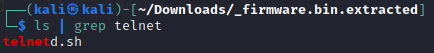
\includegraphics[scale=0.5]{telnet.png}
\end{center}
In there we can find the username 'Device\_Admin' and a hint for the password, which lays in the file 'sign' that can be found within the file system.
\begin{center}
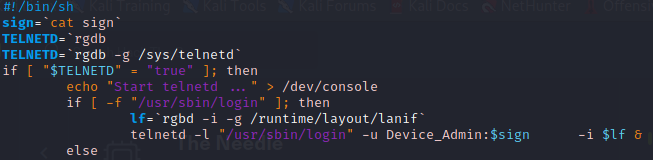
\includegraphics[scale=0.5]{telnetf.png} 
\end{center}
\newpage
After connecting to the telnet service, we find the flag there.
\begin{center}
 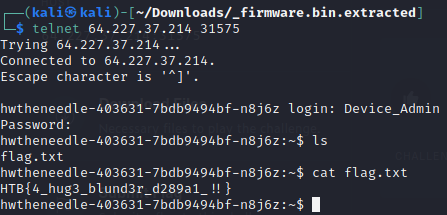
\includegraphics[scale=0.5]{flag.png}
\end{center}
\subsection{Password Cracking - Timing Side Channel Attack}



\end{document}
